\chapter{PROPUESTA Y DESARROLLO DE LA SOLUCIÓN}
\label{ch:propuesta-desarrollo}
\thispagestyle{empty}

Este capítulo expone la formulación explícita del artefacto computacional, el diseño experimental registrado antes de la búsqueda numérica, los resultados de la campaña ejecutada y la delimitación del dominio de aceptación. Las campañas previas basadas en suelo perforado y reconstrucción radial se conservan en el expediente histórico, sin sumarse a la evaluación de esta formulación. Cualquier modificación del modelo físico obliga a generar nuevas referencias FEM y a recalificar las redes neuronales correspondientes.

\section{PRESENTACIÓN DE LA PROPUESTA DE SOLUCIÓN}
\label{sec:presentacion-propuesta}

El artefacto propuesto integra un contrato físico común, un solucionador PINN por subdominios materiales, una referencia independiente en FEniCSx y un expediente trazable por ejecución. La distribución de temperatura se resuelve explícitamente en el interior del conductor, el aislamiento, la pantalla, la cubierta y el suelo circundante. Cada región satisface su propia ecuación diferencial y las interfaces transmiten la temperatura y el flujo térmico normal. En consecuencia, no se impone una potencia uniforme en la superficie externa del cable ni se añade una caída térmica resistiva equivalente para inferir la temperatura del conductor.

La contribución desde el enfoque de ciencia del diseño reside en el procedimiento de especificación, selección controlada, verificación independiente y delimitación explícita del artefacto \parencites{peffers2007}{gregor2013}. La aprobación de un protocolo autoriza la fase experimental, pero no certifica automáticamente todas las configuraciones ni todos los casos del catálogo. Cada red se entrena para un problema físico particular, de modo que el artefacto no constituye un operador capaz de generalizar sin reentrenamiento hacia geometrías o propiedades térmicas distintas.

\section{DESARROLLO DE LA PROPUESTA DE SOLUCIÓN}
\label{sec:desarrollo-solucion}

\subsection{CONTRATO FÍSICO Y CATÁLOGO DE CASOS}

Los archivos JSON en codificación UTF-8 especifican el contrato físico de cada caso. Dichos archivos registran la geometría del dominio, los centros y radios de las capas, la conductividad de cada material, la ley espacial del suelo, la fuente, la resistencia, el coeficiente térmico y los contornos. Las longitudes se expresan en metros, la conductividad térmica $k$ en \si{\watt\per\metre\per\kelvin}, la generación volumétrica $Q$ en \si{\watt\per\metre\cubed}, la potencia lineal en \si{\watt\per\metre} y las diferencias de temperatura en kelvin. Los hiperparámetros numéricos y las semillas aleatorias se alojan en archivos separados y no alteran la identidad física del caso.

Los cables del catálogo utilizan el dominio rectangular $[-4,4]\times[-4,0]$ m y una temperatura prescrita de \SI{20}{\celsius} en el contorno exterior. Este borde finito forma parte integral del problema, por lo que la convergencia de malla no demuestra por sí sola independencia frente a la extensión del terreno. Cuando se requiera ampliar el dominio en futuras evaluaciones, el protocolo del plan establece duplicar las distancias laterales y de fondo hasta que el cambio en $\Tmax$ no supere \SI{0,05}{\kelvin} y la variación de ampacidad no supere el 0,2\,\pct{}. Como control geométrico reducido, el caso coaxial emplea un círculo de radio \SI{0,15}{\metre}, cuya variante angular prescribe $T=20+10x$ en el contorno (con $x$ en metros) para evitar seleccionar una representación únicamente por su comportamiento en simetría radial.

La familia de cable XLPE monocapa o multicapa presenta un radio del conductor de \SI{5,5}{\milli\metre} y un radio exterior de \SI{15}{\milli\metre}. Esta familia abarca suelo homogéneo, estratos horizontales con salto discontinuo de conductividad, relleno mejorado y zonas secas de baja conductividad cercana y lejana. El caso Aras incorpora un arreglo plano de tres cables y el caso Kim modela seis cables enterrados en arena. Estas disposiciones geométricas se inspiran en \textcite{aras2005} y \textcite{kim2025}, aunque el dominio rectangular, las fuentes prescritas y los contornos controlados del contrato no reproducen íntegramente aquellas instalaciones. El año 2024 presente en rutas históricas del caso Kim responde a una convención de carpeta, mientras que la cita bibliográfica corresponde al año 2025. Además, se adopta el coeficiente térmico estándar de \SI{0,00393}{\per\kelvin}, documentando la discrepancia respecto al valor 0,0393 impreso en el antecedente heredado.

En relación con el catálogo mínimo planteado en el diseño inicial del plan de tesis, la campaña explícita ejecutada cubre ocho casos de referencia que articulan la verificación analítica, el control de transición suave y los arreglos multicapa enterrados. En particular, el control coaxial radial y el coaxial angular cumplen la función de verificación analítica del solucionador equivalente al anillo A1 del plan, mientras que el arreglo \texttt{aras\_flat} corresponde a la configuración plana C0 adaptada de \textcite{aras2005}. Por su parte, la disposición sintética en trébol (C1) y la grilla paramétrica completa de veinticuatro combinaciones de $w/D\in\{2,4\}$, $d_h/D\in\{0{,}5;2\}$ y $k_h/k_{\mathrm{nativo}}\in\{0{,}25;0{,}5;2;4\}$ permanecen especificadas como extensiones metodológicas fuera de las ejecuciones completadas.

Una transición de conductividad suavizada y una interfaz con salto exacto definen problemas matemáticos distintos. Por ello, el ancho de transición se registra como propiedad física del caso y no se modifica para facilitar la convergencia del entrenamiento. El validador previo rechaza geometrías superpuestas, capas discontinuas en radio, conductividades no positivas y estratos que intercepten físicamente un cable cuando el generador de malla no soporta dicha intersección.

La resistencia eléctrica exige identificar si su base es DC o AC, junto con su frecuencia, temperatura de referencia y fuente primaria. Los valores históricos rotulados como $R_{20}$ se tratan como resistencia DC dentro de los controles declarados, dado que esa etiqueta no certifica por sí misma el régimen original del dato. La campaña principal compara fuentes térmicas prescritas, mientras que la ley DC local acoplada a la temperatura y la búsqueda de corriente límite se especifican en módulos separados sin transferir cifras de ampacidad de formulaciones reducidas previas. Las Tablas~\ref{tab:explicit-case-inputs}, \ref{tab:explicit-layers} y~\ref{tab:explicit-patches} reúnen, respectivamente, las entradas eléctricas y térmicas base, las capas explícitas del cable y los parches de heterogeneidad del suelo.

\begingroup\footnotesize\setlength{\tabcolsep}{3pt}
\begin{longtable}{L{4.2cm}rrrrr}
\caption{Entradas eléctricas y del suelo base de la campaña a fuente prescrita. Fuente: contratos de caso documentados.}\label{tab:explicit-case-inputs}\\
\toprule
Caso & Cables & I, A & $R_{20}$, $\Omega$/km & P por cable, W/m & k base, W/(m K)\\
\midrule\endfirsthead
\toprule
Caso & Cables & I, A & $R_{20}$, $\Omega$/km & P por cable, W/m & k base, W/(m K)\\
\midrule\endhead
coaxial\_angular & 1 & 270 & 0.19300 & 14.06970 & 1.000\\
xlpe\_single & 1 & 270 & 0.19300 & 14.06970 & 1.000\\
xlpe\_discrete\_layers & 1 & 270 & 0.19300 & 14.06970 & 1.000\\
xlpe\_backfill & 1 & 270 & 0.19300 & 14.06970 & 1.000\\
xlpe\_dry\_near & 1 & 270 & 0.19300 & 14.06970 & 1.000\\
xlpe\_dry\_far & 1 & 270 & 0.19300 & 14.06970 & 1.000\\
aras\_flat & 3 & 1110 & 0.01510 & 18.60471 & 1.000\\
kim\_sand & 6 & 1026 & 0.01510 & 15.89541 & 1.365\\
\bottomrule\end{longtable}\endgroup

\begingroup\footnotesize\setlength{\tabcolsep}{3pt}
\begin{longtable}{L{4.2cm}rrrrr}
\caption{Capas explícitas: índice cero conductor, los restantes materiales pasivos. Fuente: fichas de entrada auditadas.}\label{tab:explicit-layers}\\
\toprule
Familia & Capa & $r_i$, mm & $r_o$, mm & Espesor, mm & k, W/(m K)\\
\midrule\endfirsthead
\toprule
Familia & Capa & $r_i$, mm & $r_o$, mm & Espesor, mm & k, W/(m K)\\
\midrule\endhead
xlpe\_single & 0 & 0.00 & 5.50 & 5.50 & 400\\
xlpe\_single & 1 & 5.50 & 12.00 & 6.50 & 0.286\\
xlpe\_single & 2 & 12.00 & 13.00 & 1.00 & 380\\
xlpe\_single & 3 & 13.00 & 15.00 & 2.00 & 0.45\\
aras\_flat & 0 & 0.00 & 18.85 & 18.85 & 400\\
aras\_flat & 1 & 18.85 & 40.85 & 22.00 & 0.2857\\
aras\_flat & 2 & 40.85 & 49.35 & 8.50 & 384.6\\
aras\_flat & 3 & 49.35 & 53.35 & 4.00 & 0.45\\
kim\_sand & 0 & 0.00 & 21.20 & 21.20 & 400\\
kim\_sand & 1 & 21.20 & 23.20 & 2.00 & 0.2857\\
kim\_sand & 2 & 23.20 & 40.20 & 17.00 & 0.2857\\
kim\_sand & 3 & 40.20 & 41.50 & 1.30 & 0.2857\\
kim\_sand & 4 & 41.50 & 42.50 & 1.00 & 0.167\\
kim\_sand & 5 & 42.50 & 45.00 & 2.50 & 237\\
kim\_sand & 6 & 45.00 & 50.00 & 5.00 & 0.2857\\
kim\_sand & 7 & 50.00 & 100.00 & 50.00 & 2.15\\
kim\_sand & 8 & 100.00 & 110.00 & 10.00 & 0.2857\\
\bottomrule\end{longtable}\endgroup

Los casos coaxial y XLPE comparten la secuencia radial de XLPE. El centro coaxial es (0,0); XLPE está en (0,−0,7) m. Aras utiliza centros (−0,33;−1,2), (0;−1,2) y (0,33;−1,2) m. Kim utiliza x=−0,4, 0 y 0,4 m en dos filas y=−1,6 y −1,2 m. Las capas de Kim se conservan individualmente aunque algunas tengan igual conductividad. No se homogeneiza su difusión térmica.

Las zonas suaves emplean $k(x,y)=k_0+(k_p-k_0)S_\varepsilon(x;c_x,w)S_\varepsilon(y;c_y,h)$, donde $S_\varepsilon(s;c,w)=\tfrac12[\tanh((s-c+w/2)/\varepsilon)-\tanh((s-c-w/2)/\varepsilon)]$. El mapa se evalúa únicamente en suelo; las capas conservan su k.

\begingroup\footnotesize\setlength{\tabcolsep}{3pt}
\begin{longtable}{L{4.2cm}rrrrrr}
\caption{Definición de heterogeneidades suaves del suelo. Fuente: casos registrados.}\label{tab:explicit-patches}\\
\toprule
Caso & $c_x$, m & $c_y$, m & w, m & h, m & $k_p$ & $\varepsilon$, m\\
\midrule\endfirsthead
\toprule
Caso & $c_x$, m & $c_y$, m & w, m & h, m & $k_p$ & $\varepsilon$, m\\
\midrule\endhead
xlpe\_backfill & 0 & -0.7 & 0.5 & 0.5 & 2 & 0.08\\
xlpe\_dry\_near & 0 & -0.7 & 0.5 & 0.5 & 0.5 & 0.08\\
xlpe\_dry\_far & 1 & -0.7 & 0.5 & 0.5 & 0.5 & 0.08\\
\bottomrule\end{longtable}\endgroup

Los estratos emplean k=0,5 W/(m K) bajo y=−1 m y k=1 W/(m K) sobre esa interfaz, con salto exacto. Los demás casos de esta tabla no tienen bandas adicionales. Las resistencias de los controles se interpretan como DC a 20 °C; el coeficiente térmico es 0,00393 $\mathrm{K}^{-1}$. La frase histórica «flujo circular uniforme» que subsiste en la procedencia del catálogo describe su uso anterior; el contrato explícito y la pérdida activa utilizan generación volumétrica y transmisión entre materiales.


\subsection{ECUACIONES Y REPRESENTACIÓN MULTIESCALA}

Dentro de cada material $i$, la ecuación estacionaria del calor en derivadas parciales adopta la forma $-\nabla\cdot(k_i\nabla T_i)=Q_i$. En el conductor $Q_i$ representa la densidad volumétrica de generación eléctrica, mientras que en las capas pasivas y en el suelo vale cero. Las derivadas espaciales de $k(x,y)$ se preservan íntegras en las regiones con conductividad continua. Sobre cada interfaz compartida, una misma normal unitaria evalúa la continuidad de la temperatura y la continuidad del flujo normal $\mathbf{q}\cdot\mathbf{n}$, en tanto que la condición exterior de Dirichlet se impone de forma exacta mediante la función de ensayo.

Las capas anulares incorporan la coordenada logradial y los términos angulares periódicos detallados en la Sección~\ref{subsec:generacion-evacuacion-calor} del Capítulo~\ref{ch:marco-teorico}. La red del conductor emplea coordenadas cartesianas normalizadas por su radio exterior, y la red del suelo combina coordenadas globales normalizadas con distancias locales hacia cada cable. Dado que las derivadas automáticas se evalúan respecto de las coordenadas físicas originales, se conservan todos los factores métricos y de escala sin reducir el problema bidimensional a una ecuación radial unidimensional.

Cada subred material produce una corrección escalada por la referencia térmica local junto con un desplazamiento entrenable. En la variante mixta de temperatura y flujo, la red calcula simultáneamente el campo escalar y el vector de flujo, imponiendo la ley de Fourier en el interior y en las trazas de frontera. No obstante, los criterios de aceptación verifican siempre el flujo derivado directamente de $-k\nabla T$, evitando que un campo de flujo auxiliar enmascare un perfil térmico físicamente inconsistente.

\begin{formula}[htbp]
\begin{equation}
\mathcal L=\mathcal L_{\mathrm{PDE}}+\mathcal L_{\mathrm{constitutiva}}
+w_T\mathcal L_{[T]}+10\mathcal L_{[q_n]}+10\mathcal L_{\mathrm{energía}}.
\label{for:perdida-explicita}
\end{equation}
\caption{Pérdida adimensional común de la campaña explícita. Fuente: Elaboración propia.}
\end{formula}

En la Fórmula~\ref{for:perdida-explicita}, el término constitutivo solo interviene cuando el flujo es una variable de salida independiente. El balance energético se integra numéricamente por región a partir de las fuentes y los flujos calculados, sin sustituir los flujos de borde por la potencia prescrita. Los residuos medios se evalúan por material para impedir que el aislamiento de menor área quede subrepresentado frente al suelo extenso. Las etapas A, B y C mantienen el peso de continuidad térmica $w_T=100$ y las restantes ponderaciones fijas, mientras que la etapa C2 varía exclusivamente $w_T$ antes de la confirmación. Ninguna temperatura de referencia FEM interviene en la función de pérdida durante el entrenamiento.

\subsection{REFERENCIA FEM Y PUERTA DE DISCRETIZACIÓN}
\label{subsec:referencia-fem}

El solucionador independiente emplea FEniCSx 0.10.0 y Gmsh 4.15.2 sobre mallas conformes con elementos triangulares cuadráticos (P2) y fronteras curvas exactas \parencite{baratta2023dolfinx}. Cada capa material recibe un marcador propio de integración y su conductividad térmica declarada, integrando la fuente volumétrica sobre la sección conductora y conservando las interfaces en el interior de la malla. El sistema algebraico resultante se resuelve mediante el método directo PETSc/MUMPS, interrumpiendo la generación de referencia ante cualquier fallo de convergencia numérica.

Para cada problema físico se ejecutan entre tres y cinco mallas sucesivamente refinadas. El tamaño local de elemento escala con el espesor de cada capa del cable y preserva la resolución en la vecindad de los parches del suelo. La puerta de discretización exige, entre los dos últimos refinamientos, una variación de $\Tmax$ menor que \SI{0,1}{\kelvin} y menor que 0,5\,\pct{} de la elevación térmica total, un cambio cuadrático medio por material inferior al 0,5\,\pct{} de esa elevación y un desequilibrio energético global menor al 0,2\,\pct{}. Estos umbrales son más estrictos que las tolerancias de la PINN, aunque la estabilidad observada entre mallas representa evidencia de convergencia numérica y no una cota analítica exacta.

La evaluación independiente utiliza 512 puntos por subdominio material, incluyendo el centro del conductor, y calcula tanto el RMSE por material como el RMSE global ponderado por área. La rutina de interpolación identifica primero el marcador geométrico de la subregión y evalúa posteriormente la celda en coordenadas isoparamétricas, evitando así errores espurios en fronteras curvas detectados durante pruebas piloto tempranas. Todos los campos comparados se evalúan en coordenadas idénticas y verifican coincidencia de huella SHA-256 en la especificación física. En el caso coaxial simétrico, la comparación externa contra la solución analítica de Poisson arrojó en la malla P2 fina un error de $\Tmax$ cercano a $3,68\times10^{-6}$ K; dicha exactitud radial no reemplaza el estudio de malla en problemas angulares y heterogéneos.

\subsection{SELECCIÓN DE ARQUITECTURA Y TAMAÑO}
\label{sec:seleccion-pinn}

La etapa de selección distingue explícitamente entre formulación física, representación de entradas y tamaño de red. El espacio evaluado abarca redes de temperatura por subdominios, redes mixtas de temperatura y flujo, entradas cartesianas locales, características de Fourier y enriquecimiento multipolar \parencite{wang2020fourier}. Los identificadores internos \texttt{enriched}, \texttt{conservative} y \texttt{subdomain} presentes en scripts previos corresponden a alias técnicos y no representan métodos numéricos distintos. Una única red global continua se descarta como control negativo debido a la imposibilidad de representar derivadas normales discontinuas cuando cambia $k(x,y)$ bajo flujo no nulo.

La variante mixta se inspira conceptualmente en las formulaciones de primer orden FO-PINNs \parencite{gladstone2022fopinn}, sin pretender reproducir exactamente los ajustes de aquel estudio. De modo análogo, el enriquecimiento multipolar introduce funciones armónicas regulares en el entorno del primer conductor, lo cual limita su simetría en configuraciones multicable. Otras estrategias bibliográficas como las formulaciones variacionales VPINN, la descomposición con ventanas solapadas FBPINN y la ponderación adaptativa de gradientes se consideran antecedentes de diseño fuera del conjunto entrenado en esta campaña \parencites{kharazmi2020hpvpinn}{moseley2021fbpinn}{wang2020gradients}.

La etapa A contrasta nueve arquitecturas: redes por subdominio de anchura y profundidad $8\times2$, $16\times2$, $16\times3$ y $32\times3$; formulaciones mixtas $16\times2$ y $32\times3$; y variantes local, Fourier y multipolar de $16\times2$. Todas las redes utilizan activación tangente hiperbólica, inicialización reproducible y precisión de punto flotante de 64 bits. Cada candidato recibe 1200 pasos del optimizador Adam con tasa de aprendizaje $10^{-3}$, seguidos de hasta 2000 iteraciones de L-BFGS con búsqueda lineal, registrando en cada corrida las evaluaciones reales ejecutadas.

Los problemas de desarrollo de la etapa A son el caso coaxial angular y el cable XLPE en suelo homogéneo. Se emplean las parejas fijas de inicialización y muestreo $(11, 101)$ y $(23, 103)$, lo que permite comparaciones pareadas entre arquitecturas aunque no descompone estadísticamente la varianza debida a los pesos iniciales frente a la varianza de colocación. El presupuesto base consta de 256 puntos en el suelo, 128 puntos por capa del cable y 96 puntos por interfaz.

La regla de selección da prioridad a las arquitecturas aceptadas simultáneamente en ambos problemas y en ambas semillas de desarrollo. Entre las candidatas admisibles se prefiere aquella con menor número de parámetros entrenables, resolviendo empates según el menor error normalizado máximo. Si ninguna candidata supera todos los criterios, se selecciona provisionalmente la configuración con mayor conteo de aceptaciones y menor violación relativa máxima. Debido al carácter discreto de la exploración y al presupuesto finito, los resultados identifican la menor red admisible dentro del conjunto ensayado sin excluir arquitecturas que podrían converger bajo presupuestos distintos \parencite{bergstra2012random}.

\subsection{CONVERGENCIA Y DISTRIBUCIÓN DE COLOCACIONES}
\label{sec:analisis-numerico-pinn}
\label{sec:muestreo-adaptativo}

La etapa B mantiene la arquitectura seleccionada en la etapa anterior y compara el caso XLPE homogéneo con el caso XLPE en estratos discontinuos. La incorporación de una interfaz horizontal en el terreno permite verificar si el presupuesto de muestreo elegido en suelo uniforme conserva su desempeño en presencia de un salto de conductividad extenso. Se mantienen exactamente las dos parejas de semillas de desarrollo empleadas en la etapa A.

El esquema base combina un muestreo de cobertura global con puntos concentrados alrededor de los cables y compara presupuestos relativos de $1\times$, $2\times$ y $4\times$. Para el presupuesto intermedio $2\times$ se contrastan además la distribución uniforme, las bandas cercanas a interfaces y la adaptación residual progresiva. De este modo, el diseño experimental separa el efecto de incrementar la densidad de puntos respecto del efecto de redistribuir espacialmente una misma cantidad de colocaciones.

La estrategia por bandas retiene la mitad de los puntos con distribución uniforme y concentra la otra mitad cerca de las fronteras internas del cable y del salto de estratos. Por su parte, la estrategia adaptativa genera cuatro veces más candidatos interiores y evalúa a mitad del ciclo Adam el residuo adimensional de la PDE junto con el defecto constitutivo en variantes mixtas. Luego remuestrea sin reemplazo la mitad del presupuesto con probabilidades proporcionales al indicador, manteniendo fija la nube resultante durante L-BFGS. Este esquema se apoya en los principios descritos por \textcite{wu2022sampling}, sin afirmar una implementación literal del algoritmo RAD ni corregir la pérdida por pesos de importancia. Las fronteras e interfaces conservan siempre cuadraturas uniformes para garantizar balances energéticos consistentes.

\begin{formula}[htbp]
\begin{equation}
D_{N,2N}=100\frac{\sqrt{\sum_j w_j(T_N-T_{2N})^2/\sum_j w_j}}
{|T^F_{\max}-T_0|},\qquad
H_{N,2N}=100\frac{|T_{\max,N}-T_{\max,2N}|}{|T^F_{\max}-T_0|}.
\label{for:insensibilidad-explicita}
\end{equation}
\caption{Indicadores de insensibilidad observada al aumentar colocaciones. Fuente: Elaboración propia.}
\end{formula}

Los indicadores $D$ y $H$ de la Fórmula~\ref{for:insensibilidad-explicita} cuantifican la variación relativa tanto del campo completo como de la temperatura máxima al duplicar el presupuesto de puntos. La estabilidad respecto a la resolución se declara únicamente cuando ambos indicadores permanecen por debajo de 0,5\,\pct{} y las dos corridas superan todos los criterios de aceptación frente a FEM. Si una pareja incumple esta condición, se reporta dependencia de resolución aunque alguna corrida aislada satisfaga los umbrales de campo.

Desde una perspectiva teórica, la tasa empírica de variación frente al tamaño de muestra no equivale a un orden clásico de convergencia ni habilita extrapolación de Richardson. Los errores de aproximación, generalización por cuadratura y optimización no convexa interactúan de forma acoplada \parencites{deryck2024analysis}{mishra2020error}. En consecuencia, el contraste $1\times$--$2\times$--$4\times$ delimita únicamente el régimen de estabilidad práctica observado en el rango ensayado.

\subsection{AJUSTE DEL ENTRENAMIENTO Y CONFIRMACIÓN}

La etapa C mantiene fija la arquitectura de la etapa A y el esquema de colocación de la etapa B para evaluar tasas de aprendizaje Adam de $5\times10^{-4}$, $10^{-3}$ y $2\times10^{-3}$, ampliando el presupuesto a 1500 pasos de Adam y hasta 3000 iteraciones de L-BFGS. Dentro de esta etapa todos los candidatos comparten exactamente la misma densidad de muestreo, mientras que la variación entre la etapa A y la etapa C refleja el ajuste secuencial del procedimiento completo.

Ante la persistencia de discontinuidades térmicas en las interfaces durante la etapa B, se registró una enmienda formativa previa denominada etapa C2 antes de proceder a la confirmación final. Dicha enmienda mantiene la tasa de aprendizaje seleccionada en la etapa C y compara los pesos $w_T\in\{100, 1000, 10000\}$ sin alterar ni las ecuaciones ni las tolerancias de evaluación. La configuración $w_T=100$ reutiliza cuatro ejecuciones ya completadas de la etapa C, mientras que los dos niveles superiores añaden ocho entrenamientos adicionales. Este ajuste atiende al equilibrio entre términos competitivos de la función de pérdida señalado por \textcite{wang2020gradients}, sin implementar reponderación dinámica automática.

Sumando las etapas de desarrollo A, B, C y C2 se contabilizan 101 entrenamientos únicos registrados en el expediente completo, complementados por nueve ensayos exploratorios de corriente límite. Una vez seleccionada la configuración en la etapa C2, se congela completamente la receta junto con su huella de código para iniciar la etapa de confirmación D con tres semillas totalmente independientes de inicialización (71, 83 y 97) y muestreo (1001, 1003 y 1007). La etapa D evalúa simultáneamente los casos de desarrollo previos y cinco escenarios nuevos no vistos durante el ajuste: relleno mejorado, zona seca cercana, zona seca lejana, arreglo plano de Aras y arreglo en arena de Kim. Todas las ejecuciones de confirmación, incluidas las rechazadas, se conservan íntegramente en los resultados mediante su mediana, su rango y su fracción de aceptación.

\subsection{MÉTRICAS Y TRAZABILIDAD}

Las métricas relativas de error térmico toman como denominador la elevación térmica $\Delta T_{\mathrm{ref}}=\Tmax^F - T_0$ sobre la temperatura ambiente, evitando sesgos derivados de usar la escala Celsius absoluta. El RMSE global pondera cada punto evaluado según el área geométrica asignada en la malla de verificación. La puerta de aceptación explícita exige que el NRMSE global, el error de $\Tmax$ y el RMSE por subdominio no excedan el 5\,\pct{}, junto con balances globales y regionales no mayores al 2\,\pct{}. Adicionalmente, demanda un salto térmico de interfaz no mayor que \SI{0,1}{\kelvin} y un salto RMS de flujo normal de hasta el 1\,\pct{} de la escala vecina mayor. En las redes mixtas deben superar estos umbrales tanto el flujo predicho directamente como el flujo calculado a partir de $-k\nabla T$.

Para preservar homogeneidad en las comparaciones, el desequilibrio global divide el flujo neto exterior entre la potencia total generada, mientras que el balance regional divide el defecto de cada zona entre la potencia nominal por cable $P_0=I_0^2R_{20}$, incluso en las capas pasivas sin generación propia. Los umbrales se fijan antes de la confirmación y permanecen invariables independientemente de los resultados observados. Cada ejecución genera registros JSON autodescriptivos que encapsulan huellas SHA-256 de código y física, nubes de puntos, estados de optimización y tiempos de cómputo. A partir de estos archivos se construyen automáticamente las tablas de resultados, eliminando transcripciones manuales. El Anexo~\ref{anx:catalogo-casos} sintetiza la cobertura por etapas, el Anexo~\ref{anx:protocolo-reproduccion} detalla el contrato de archivos, el Anexo~\ref{anx:requisito-evidencia} consolida la matriz requisito--evidencia (Tabla~\ref{tab:explicit-requirements}) y el Anexo~\ref{anx:expediente-evidencia} lista las 101 ejecuciones (Tabla~\ref{tab:explicit-all}).

En cuanto al entorno de ejecución, las pruebas se desarrollaron en un equipo con procesador Intel Core Ultra 7 165U y acelerador integrado Intel sin soporte CUDA, utilizando precisión de 64 bits y un hilo por entrenamiento bajo hasta tres procesos paralelos independientes. Debido a que las subredes materiales se evalúan secuencialmente y a que no se cronometraron ejecuciones aisladas equivalentes de FEniCSx, los registros de tiempo documentan el costo computacional de la campaña sin afirmar aceleración respecto a FEM.

\subsection{ACOPLAMIENTO ELECTROTÉRMICO Y BÚSQUEDA ACOTADA DE AMPACIDAD}
\label{subsec:busqueda-ampacidad}

Para la extensión de corriente límite vinculada al cuarto objetivo específico, el artefacto incorpora la ley local dependiente de la temperatura dada por la Fórmula~\ref{for:fuente-dc-local}. Dada una corriente eficaz equilibrada $I$ idéntica en todos los conductores, el acoplamiento electrotérmico se resuelve por iteración de punto fijo iniciando la temperatura media de cada conductor $\overline{T}_{c,j}$ en $T_{\mathrm{amb}}$, evaluando las pérdidas $Q_j$ y relajando iterativamente mediante $\overline{T}_{c,j}^{\,n+1}=0{,}5\overline{T}_{c,j}^{\,n}+0{,}5\langle T^{n+1}\rangle_{c,j}$. La convergencia exige simultáneamente variaciones medias inferiores a \SI{0,001}{\kelvin}, un cambio relativo de fuente $\max_j\{|Q_j^{n+1}-Q_j^n|/\max(|Q_j^{n+1}|,Q_0)\}<10^{-4}$ en un máximo de 100 iteraciones y cumplimiento del balance energético.

Sobre ese lazo interno acoplado, el protocolo especificado en \path{Benchmarks/full_ampacity_study.py} acota la ampacidad partiendo de un límite inferior $I_L=0$ y duplicando un límite superior positivo hasta alcanzar $T_{\max}(I_L)\leq T_{\mathrm{lim}}<T_{\max}(I_U)$ en un máximo de doce ampliaciones. Una vez encerrada la raíz, se aplica bisección mediante $I_M=(I_L+I_U)/2$ hasta cumplir $(I_U-I_L)/I_U\leq10^{-3}$ y $|T_{\max}(I_M)-T_{\mathrm{lim}}|\leq\SI{0,05}{\kelvin}$ en un tope de 60 pasos, verificando el comportamiento monótono no decreciente de la temperatura frente a la corriente. Tanto la PINN como la referencia FEM ejecutan búsquedas independientes; luego, FEM evalúa los extremos y el punto medio reportados por la PINN sin transferir información al entrenamiento. Con ello se construyen intervalos ampliados con la incertidumbre térmica acumulada, exigiendo en el criterio F4 del plan un error relativo de ampacidad menor al 1\,\pct{} por semilla. Mientras la rutina quedó implementada y verificada a nivel de componente en el piloto DC coaxial, la campaña completa de búsqueda sobre pares heterogéneos y homogéneos equivalentes permanece pendiente de ejecución.

\section{ANÁLISIS DE LOS DATOS Y RESULTADOS}
\label{sec:analisis-resultados}

Los resultados siguen la secuencia cronológica de las etapas del diseño experimental. La Tabla~\ref{tab:explicit-fem} consolida las referencias FEM verificadas para los ocho casos físicos; las Tablas~\ref{tab:explicit-A} y~\ref{tab:explicit-A-diagnosis} presentan la búsqueda de arquitectura y tamaño; y las Tablas~\ref{tab:explicit-B}, \ref{tab:explicit-B-diagnosis}, \ref{tab:explicit-point-counts} y~\ref{tab:explicit-convergence} evalúan el efecto del presupuesto y la distribución de colocaciones. A continuación, las Tablas~\ref{tab:explicit-C} y~\ref{tab:explicit-C2} recogen el ajuste de tasa de aprendizaje y continuidad en interfaz; la Tabla~\ref{tab:explicit-smallest} resume la menor arquitectura aceptada por problema; y las Tablas~\ref{tab:explicit-production}, \ref{tab:explicit-effects} y~\ref{tab:explicit-effect-resolution} reportan la etapa de confirmación con semillas nuevas.

De manera complementaria, cinco figuras ilustran el comportamiento espacial y numérico de la campaña. La Figura~\ref{fig:explicit-selection} resume visualmente las aceptaciones y rechazos obtenidos a través de las etapas A, B, C y C2 de desarrollo, mientras que la Figura~\ref{fig:explicit-convergence} muestra la evolución del error respecto al incremento de puntos de colocación bajo arquitectura fija. Asimismo, las Figuras~\ref{fig:explicit-collocation-domain} y~\ref{fig:explicit-collocation-detail} exhiben las nubes de colocación a presupuesto $2\times$ sobre el dominio completo y en el entorno inmediato del cable para las cuatro políticas ensayadas. Por último, la Figura~\ref{fig:explicit-field} contrasta la distribución térmica calculada y el error espacial respecto a FEM para la zona seca cercana en confirmación con la semilla 71. Las Secciones~\ref{sec:diagnostico-rechazos}, \ref{sec:dominio-validez} y~\ref{sec:matriz-validez} analizan los fallos observados, delimitan el dominio de aceptación y establecen la matriz de validez, apoyándose en el registro integral de ejecuciones del Anexo~\ref{anx:expediente-evidencia}.

\subsection{REFERENCIAS Y COBERTURA EFECTIVA}

\begingroup\footnotesize\setlength{\tabcolsep}{3pt}
\begin{longtable}{L{4.2cm}rrrrr}
\caption{Referencias FEM explícitas refinadas. Fuente: registros de la campaña.}\label{tab:explicit-fem}\\
\toprule
Caso & Niveles & Grados de libertad & $T_{\max}$, °C & $\Delta T_{\max}$, K & Balance, \pct{}\\
\midrule\endfirsthead
\toprule
Caso & Niveles & Grados de libertad & $T_{\max}$, °C & $\Delta T_{\max}$, K & Balance, \pct{}\\
\midrule\endhead
aras\_flat & 3 & 264969 & 50.058 & 0.00349 & 0.01045\\
coaxial\_angular & 3 & 152951 & 31.980 & 0.00005 & 0.02704\\
kim\_sand & 3 & 2802105 & 49.757 & 0.00013 & 0.00805\\
xlpe\_backfill & 3 & 97221 & 33.525 & 0.01617 & 0.00673\\
xlpe\_discrete\_layers & 3 & 97217 & 37.371 & 0.03491 & 0.00156\\
xlpe\_dry\_far & 3 & 97221 & 36.889 & 0.03382 & 0.00736\\
xlpe\_dry\_near & 3 & 97221 & 42.862 & 0.07832 & 0.00741\\
xlpe\_single & 3 & 97221 & 36.852 & 0.03377 & 0.00718\\
\bottomrule\end{longtable}\endgroup

Todas las comparaciones de las etapas A--D utilizan estas referencias de la misma formulación física. El refinamiento verifica también el cambio de campo por material. La cantidad de semillas no debe confundirse con el número de instalaciones independientes.

\subsection{ARQUITECTURA Y TAMAÑO}

\begingroup\footnotesize\setlength{\tabcolsep}{3pt}
\begin{longtable}{L{4.2cm}rrrrr}
\caption{Etapa A: comparación de todas las semillas de desarrollo. Fuente: elaboración propia.}\label{tab:explicit-A}\\
\toprule
Configuración & Parámetros & Aceptadas & RMSE med., K & \makecell{Error máx.\\$T_{\max}$, K} & Violación máxima\\
\midrule\endfirsthead
\toprule
Configuración & Parámetros & Aceptadas & RMSE med., K & \makecell{Error máx.\\$T_{\max}$, K} & Violación máxima\\
\midrule\endhead
fourier\_w16\_d2 & 2202 & 0/4 & 1.090 & 16.823 & 19.965\\
local\_w16\_d2 & 1690 & 0/4 & 0.957 & 16.789 & 203.622\\
mixed\_w16\_d2 & 1924 & 0/4 & 0.548 & 12.064 & 26.087\\
mixed\_w32\_d3 & 11668 & 0/4 & 0.598 & 12.445 & 25.740\\
multipole\_w16\_d2 & 1784 & 0/4 & 0.199 & 0.221 & 7.596\\
subdomain\_w16\_d2 & 1754 & 2/4 & 0.213 & 0.784 & 5.075\\
subdomain\_w16\_d3 & 3114 & 0/4 & 0.269 & 0.909 & 9.241\\
subdomain\_w32\_d3 & 11338 & 3/4 & 0.195 & 0.511 & 1.560\\
subdomain\_w8\_d2 & 562 & 0/4 & 0.274 & 0.908 & 9.397\\
\bottomrule\end{longtable}\endgroup

La regla registrada selecciona \texttt{subdomain\_w32\_d3}. La selección es provisional: ninguna candidata cumple en todos los problemas y semillas de la etapa. No se declara una red o receta mínima admisible.

La violación máxima es el mayor cociente entre una métrica de rechazo y su tolerancia; un valor mayor que uno identifica incumplimiento. Las medianas incluyen también los intentos rechazados. Los parámetros corresponden al mayor tamaño total entre los casos de la etapa.

\begingroup\footnotesize\setlength{\tabcolsep}{3pt}
\begin{longtable}{L{5.2cm}L{4cm}r}
\caption{Mayor restricción relativa de la etapa A, incluidos los intentos rechazados. Fuente: elaboración propia.}\label{tab:explicit-A-diagnosis}\\
\toprule
Configuración & Restricción dominante & Cociente\\
\midrule\endfirsthead
\toprule
Configuración & Restricción dominante & Cociente\\
\midrule\endhead
fourier\_w16\_d2 & Tmax & 19.965\\
local\_w16\_d2 & Salto T & 203.622\\
mixed\_w16\_d2 & Salto flujo & 26.087\\
mixed\_w32\_d3 & Salto flujo & 25.740\\
multipole\_w16\_d2 & Salto T & 7.596\\
subdomain\_w16\_d2 & Salto T & 5.075\\
subdomain\_w16\_d3 & Salto T & 9.241\\
subdomain\_w32\_d3 & Salto T & 1.560\\
subdomain\_w8\_d2 & Salto T & 9.397\\
\bottomrule\end{longtable}\endgroup

La restricción dominante identifica dónde se incumple más la tolerancia, no demuestra por sí sola la causa de optimización.

La formulación mixta añade variables y ecuaciones; su rechazo con este presupuesto no refuta su equivalencia física. La comparación de Fourier conserva frecuencias fijadas y no optimiza su espectro. La variante multipolar ensayada tampoco agota todas las bases posibles.

\subsection{COLOCACIONES Y LOCALIZACIÓN}

\begingroup\footnotesize\setlength{\tabcolsep}{3pt}
\begin{longtable}{L{4.2cm}rrrrr}
\caption{Etapa B: comparación de todas las semillas de desarrollo. Fuente: elaboración propia.}\label{tab:explicit-B}\\
\toprule
Configuración & Parámetros & Aceptadas & RMSE med., K & \makecell{Error máx.\\$T_{\max}$, K} & Violación máxima\\
\midrule\endfirsthead
\toprule
Configuración & Parámetros & Aceptadas & RMSE med., K & \makecell{Error máx.\\$T_{\max}$, K} & Violación máxima\\
\midrule\endhead
interface\_2x & 13612 & 2/4 & 0.420 & 1.886 & 7.022\\
mixed\_1x & 13612 & 2/4 & 0.360 & 0.590 & 6.365\\
mixed\_2x & 13612 & 2/4 & 0.347 & 0.623 & 5.048\\
mixed\_4x & 13612 & 2/4 & 0.411 & 0.803 & 6.527\\
residual\_2x & 13612 & 2/4 & 0.332 & 0.940 & 6.257\\
uniform\_2x & 13612 & 0/4 & 0.459 & 6.920 & 8.213\\
\bottomrule\end{longtable}\endgroup

La regla registrada selecciona \texttt{mixed\_2x}. La selección es provisional: ninguna candidata cumple en todos los problemas y semillas de la etapa. No se declara una red o receta mínima admisible.

La violación máxima es el mayor cociente entre una métrica de rechazo y su tolerancia; un valor mayor que uno identifica incumplimiento. Las medianas incluyen también los intentos rechazados. Los parámetros corresponden al mayor tamaño total entre los casos de la etapa.

\begingroup\footnotesize\setlength{\tabcolsep}{3pt}
\begin{longtable}{L{5.2cm}L{4cm}r}
\caption{Mayor restricción relativa de la etapa B, incluidos los intentos rechazados. Fuente: elaboración propia.}\label{tab:explicit-B-diagnosis}\\
\toprule
Configuración & Restricción dominante & Cociente\\
\midrule\endfirsthead
\toprule
Configuración & Restricción dominante & Cociente\\
\midrule\endhead
interface\_2x & Salto T & 7.022\\
mixed\_1x & Salto T & 6.365\\
mixed\_2x & Salto T & 5.048\\
mixed\_4x & Salto T & 6.527\\
residual\_2x & Salto T & 6.257\\
uniform\_2x & Tmax & 8.213\\
\bottomrule\end{longtable}\endgroup

La restricción dominante identifica dónde se incumple más la tolerancia, no demuestra por sí sola la causa de optimización.

Un balance integral pequeño puede coexistir con errores del campo o de las interfaces. La nube uniforme deja pocas muestras próximas al cable dentro de un suelo extenso; se evalúa su consecuencia mediante FEM, sin considerar suficiente una pérdida de entrenamiento pequeña.

\subsection{AJUSTE DE ENTRENAMIENTO}

\begingroup\footnotesize\setlength{\tabcolsep}{3pt}
\begin{longtable}{L{4.2cm}rrrrr}
\caption{Etapa C: comparación de todas las semillas de desarrollo. Fuente: elaboración propia.}\label{tab:explicit-C}\\
\toprule
Configuración & Parámetros & Aceptadas & RMSE med., K & \makecell{Error máx.\\$T_{\max}$, K} & Violación máxima\\
\midrule\endfirsthead
\toprule
Configuración & Parámetros & Aceptadas & RMSE med., K & \makecell{Error máx.\\$T_{\max}$, K} & Violación máxima\\
\midrule\endhead
lr\_0.0005 & 13612 & 2/4 & 0.419 & 0.581 & 4.487\\
lr\_0.001 & 13612 & 1/4 & 0.377 & 0.602 & 4.424\\
lr\_0.002 & 13612 & 1/4 & 0.277 & 0.195 & 5.131\\
\bottomrule\end{longtable}\endgroup

La regla registrada selecciona \texttt{lr\_0.0005}. La selección es provisional: ninguna candidata cumple en todos los problemas y semillas de la etapa. No se declara una red o receta mínima admisible.

La violación máxima es el mayor cociente entre una métrica de rechazo y su tolerancia; un valor mayor que uno identifica incumplimiento. Las medianas incluyen también los intentos rechazados. Los parámetros corresponden al mayor tamaño total entre los casos de la etapa.

\subsection{CALIBRACIÓN ADICIONAL DE CONTINUIDAD TÉRMICA}

Esta ampliación se registró durante B, antes de C y de toda confirmación, al persistir saltos térmicos excesivos con refinamiento de puntos. Cambia únicamente el peso de continuidad de temperatura; conserva las ecuaciones, normalizaciones y tolerancias. El peso 100 reutiliza cuatro ejecuciones de C; 1000 y 10000 añaden ocho entrenamientos. Las corridas reutilizadas no se cuentan dos veces en el total.

\begingroup\footnotesize\setlength{\tabcolsep}{3pt}
\begin{longtable}{L{4.2cm}rrrrr}
\caption{Etapa C2: comparación de todas las semillas de desarrollo. Fuente: elaboración propia.}\label{tab:explicit-C2}\\
\toprule
Configuración & Parámetros & Aceptadas & RMSE med., K & \makecell{Error máx.\\$T_{\max}$, K} & Violación máxima\\
\midrule\endfirsthead
\toprule
Configuración & Parámetros & Aceptadas & RMSE med., K & \makecell{Error máx.\\$T_{\max}$, K} & Violación máxima\\
\midrule\endhead
weight\_100 & 13612 & 2/4 & 0.419 & 0.581 & 4.487\\
weight\_1000 & 13612 & 2/4 & 0.345 & 0.676 & 1.595\\
weight\_10000 & 13612 & 2/4 & 0.276 & 0.477 & 2.075\\
\bottomrule\end{longtable}\endgroup

La regla registrada selecciona \texttt{weight\_1000}. La selección es provisional: ninguna candidata cumple en todos los problemas y semillas de la etapa. No se declara una red o receta mínima admisible.

La violación máxima es el mayor cociente entre una métrica de rechazo y su tolerancia; un valor mayor que uno identifica incumplimiento. Las medianas incluyen también los intentos rechazados. Los parámetros corresponden al mayor tamaño total entre los casos de la etapa.

\subsection{MENOR RED POR PROBLEMA DENTRO DEL ESPACIO ENSAYADO}

\begingroup\footnotesize\setlength{\tabcolsep}{3pt}
\begin{longtable}{L{3.5cm}L{4.2cm}rr}
\caption{Menor red aceptada por problema entre las candidatas de A. No es una garantía fuera del caso ensayado. Fuente: elaboración propia.}\label{tab:explicit-smallest}\\
\toprule
Problema & Menor candidata & Parámetros & RMSE med., K\\
\midrule\endfirsthead
\toprule
Problema & Menor candidata & Parámetros & RMSE med., K\\
\midrule\endhead
coaxial\_angular & Ninguna & -- & --\\
xlpe\_single & subdomain\_w16\_d2 & 1754 & 0.381\\
\bottomrule\end{longtable}\endgroup

\subsection{INSENSIBILIDAD Y PRESUPUESTOS DE COLOCACIÓN}

\begingroup\footnotesize\setlength{\tabcolsep}{3pt}
\begin{longtable}{L{4.2cm}rrrr}
\caption{Colocaciones efectivas por problema y factor. Las interfaces tienen dos trazas en una misma posición. Fuente: elaboración propia.}\label{tab:explicit-point-counts}\\
\toprule
Caso & Factor & Interior suelo & Interior cable & Interfaces\\
\midrule\endfirsthead
\toprule
Caso & Factor & Interior suelo & Interior cable & Interfaces\\
\midrule\endhead
xlpe\_single & 1x & 256 & 512 & 384\\
xlpe\_single & 2x & 512 & 1024 & 768\\
xlpe\_single & 4x & 1024 & 2048 & 1536\\
xlpe\_discrete\_layers & 1x & 512 & 512 & 480\\
xlpe\_discrete\_layers & 2x & 1024 & 1024 & 960\\
xlpe\_discrete\_layers & 4x & 2048 & 2048 & 1920\\
\bottomrule\end{longtable}\endgroup

Las políticas uniforme, de interfaz y residual se comparan con el presupuesto 2x. Estos conteos excluyen las cuadraturas auxiliares: cada lado exterior emplea 96 veces el factor y cada conductor usa el máximo entre 256 y 128 veces el factor para la integral eléctrica, activa en DC. Por ello, el contraste 1x--4x aumenta el presupuesto espacial conjunto, no aísla solo los puntos interiores. No se interpreta la suma como una malla FEM ni se cuenta cada traza de interfaz como una posición nueva.

\begingroup\footnotesize\setlength{\tabcolsep}{3pt}
\begin{longtable}{L{4.2cm}rrrrr}
\caption{Insensibilidad observada al aumentar colocaciones. Ambos cálculos deben estar aceptados. Fuente: elaboración propia.}\label{tab:explicit-convergence}\\
\toprule
Caso & Semilla & Cambio & $D$, \pct{} & $H$, \pct{} & Insensible\\
\midrule\endfirsthead
\toprule
Caso & Semilla & Cambio & $D$, \pct{} & $H$, \pct{} & Insensible\\
\midrule\endhead
xlpe\_single & 11 & 1x--2x & 1.979 & 0.913 & No\\
xlpe\_single & 11 & 2x--4x & 1.904 & 1.790 & No\\
xlpe\_single & 23 & 1x--2x & 1.376 & 0.392 & No\\
xlpe\_single & 23 & 2x--4x & 2.261 & 2.915 & No\\
xlpe\_discrete\_layers & 11 & 1x--2x & 1.514 & 0.189 & No\\
xlpe\_discrete\_layers & 11 & 2x--4x & 0.457 & 0.732 & No\\
xlpe\_discrete\_layers & 23 & 1x--2x & 3.056 & 1.028 & No\\
xlpe\_discrete\_layers & 23 & 2x--4x & 1.770 & 1.756 & No\\
\bottomrule\end{longtable}\endgroup

Se cumple la comprobación de insensibilidad en 0 de 8 comparaciones. Las diferencias restantes impiden afirmar independencia universal del número de colocaciones.

Este contraste corresponde al presupuesto y pesos de B. El ajuste posterior de C y C2 no convierte retrospectivamente esos pares en convergentes ni demuestra independencia de colocaciones de la receta final. La aceptación de D se refiere a errores y criterios físicos evaluados frente a FEM con el presupuesto congelado.

\subsection{CONFIRMACIÓN CON SEMILLAS INDEPENDIENTES}

\begingroup\footnotesize\setlength{\tabcolsep}{3pt}
\begin{longtable}{L{3.4cm}rrrrr}
\caption{Confirmación de la receta congelada: semillas 71, 83 y 97. Fuente: elaboración propia.}\label{tab:explicit-production}\\
\toprule
Caso & Aceptadas & RMSE med., K & RMSE mín.--máx., K & \makecell{Error máx.\\$T_{\max}$, K} & Balance máx., \pct{}\\
\midrule\endfirsthead
\toprule
Caso & Aceptadas & RMSE med., K & RMSE mín.--máx., K & \makecell{Error máx.\\$T_{\max}$, K} & Balance máx., \pct{}\\
\midrule\endhead
aras\_flat & 0/3 & 1.707 & 1.696--2.632 & 8.321 & 0.237\\
kim\_sand & 0/3 & 1.690 & 1.625--2.495 & 8.558 & 2.680\\
xlpe\_backfill & 0/3 & 0.734 & 0.730--1.185 & 1.347 & 2.928\\
xlpe\_discrete\_layers & 0/3 & 0.301 & 0.163--0.474 & 0.797 & 1.046\\
xlpe\_dry\_far & 3/3 & 0.296 & 0.263--0.338 & 0.441 & 0.962\\
xlpe\_dry\_near & 1/3 & 0.733 & 0.499--0.746 & 2.474 & 1.717\\
xlpe\_single & 3/3 & 0.253 & 0.243--0.257 & 0.378 & 0.873\\
\bottomrule\end{longtable}\endgroup

Los casos aceptados parcialmente no se consideran configuraciones robustas. Ninguna semilla de confirmación se utilizó para elegir la receta de C y C2. Las diferencias de rendimiento entre casos corresponden a transferencia del procedimiento con reentrenamiento, no de una única red ya entrenada.

\begingroup\footnotesize\setlength{\tabcolsep}{3pt}
\begin{longtable}{L{4.2cm}rrr}
\caption{Efectos térmicos respecto al control XLPE homogéneo, a igual fuente prescrita. Fuente: elaboración propia.}\label{tab:explicit-effects}\\
\toprule
Escenario & $\Delta T^F_{\max}$, K & Mediana $\Delta T^P_{\max}$, K & Pares aceptados\\
\midrule\endfirsthead
\toprule
Escenario & $\Delta T^F_{\max}$, K & Mediana $\Delta T^P_{\max}$, K & Pares aceptados\\
\midrule\endhead
xlpe\_backfill & -3.327 & -4.080 & 0/3\\
xlpe\_dry\_near & 6.009 & 3.893 & 1/3\\
xlpe\_dry\_far & 0.036 & -0.089 & 3/3\\
xlpe\_discrete\_layers & 0.519 & 0.574 & 0/3\\
\bottomrule\end{longtable}\endgroup

Las diferencias FEM caracterizan los pares físicos; una diferencia PINN de un par rechazado es diagnóstica y no confirma el efecto mediante el artefacto. El control homogéneo utiliza k del suelo base, no se identifica automáticamente con un promedio equivalente del mapa heterogéneo.

\begingroup\footnotesize\setlength{\tabcolsep}{3pt}
\begin{longtable}{L{4.2cm}rrr}
\caption{Resolución empírica del efecto: discretización y variabilidad pareada. Fuente: elaboración propia.}\label{tab:explicit-effect-resolution}\\
\toprule
Caso & Cambio de malla, K & Rango PINN, K & Resuelto\\
\midrule\endfirsthead
\toprule
Caso & Cambio de malla, K & Rango PINN, K & Resuelto\\
\midrule\endhead
xlpe\_backfill & 0.01759 & 0.511 & No\\
xlpe\_dry\_near & 0.04455 & 1.854 & No\\
xlpe\_dry\_far & 0.00005 & 0.131 & No\\
xlpe\_discrete\_layers & 0.00114 & 0.814 & No\\
\bottomrule\end{longtable}\endgroup

Se exige aceptación de los tres pares, signos coincidentes con FEM y tanto rango PINN como cambio del efecto por malla menores que el módulo del efecto FEM. Esta regla se explicitó antes de D. Es una comprobación empírica de resolución, sin intervalos poblacionales ni cotas rigurosas de error.

La ubicación del máximo se conserva en el expediente sobre la nube común de conductores. El muestreo y la escasa diferencia térmica dentro del metal impiden atribuir precisión milimétrica a esa ubicación. OE3 dispone de temperaturas y efectos contrastados, pero no de una certificación del punto caliente continuo; no se confunde una máxima muestreada con una búsqueda espacial convergente.

\begin{figure}[p]\centering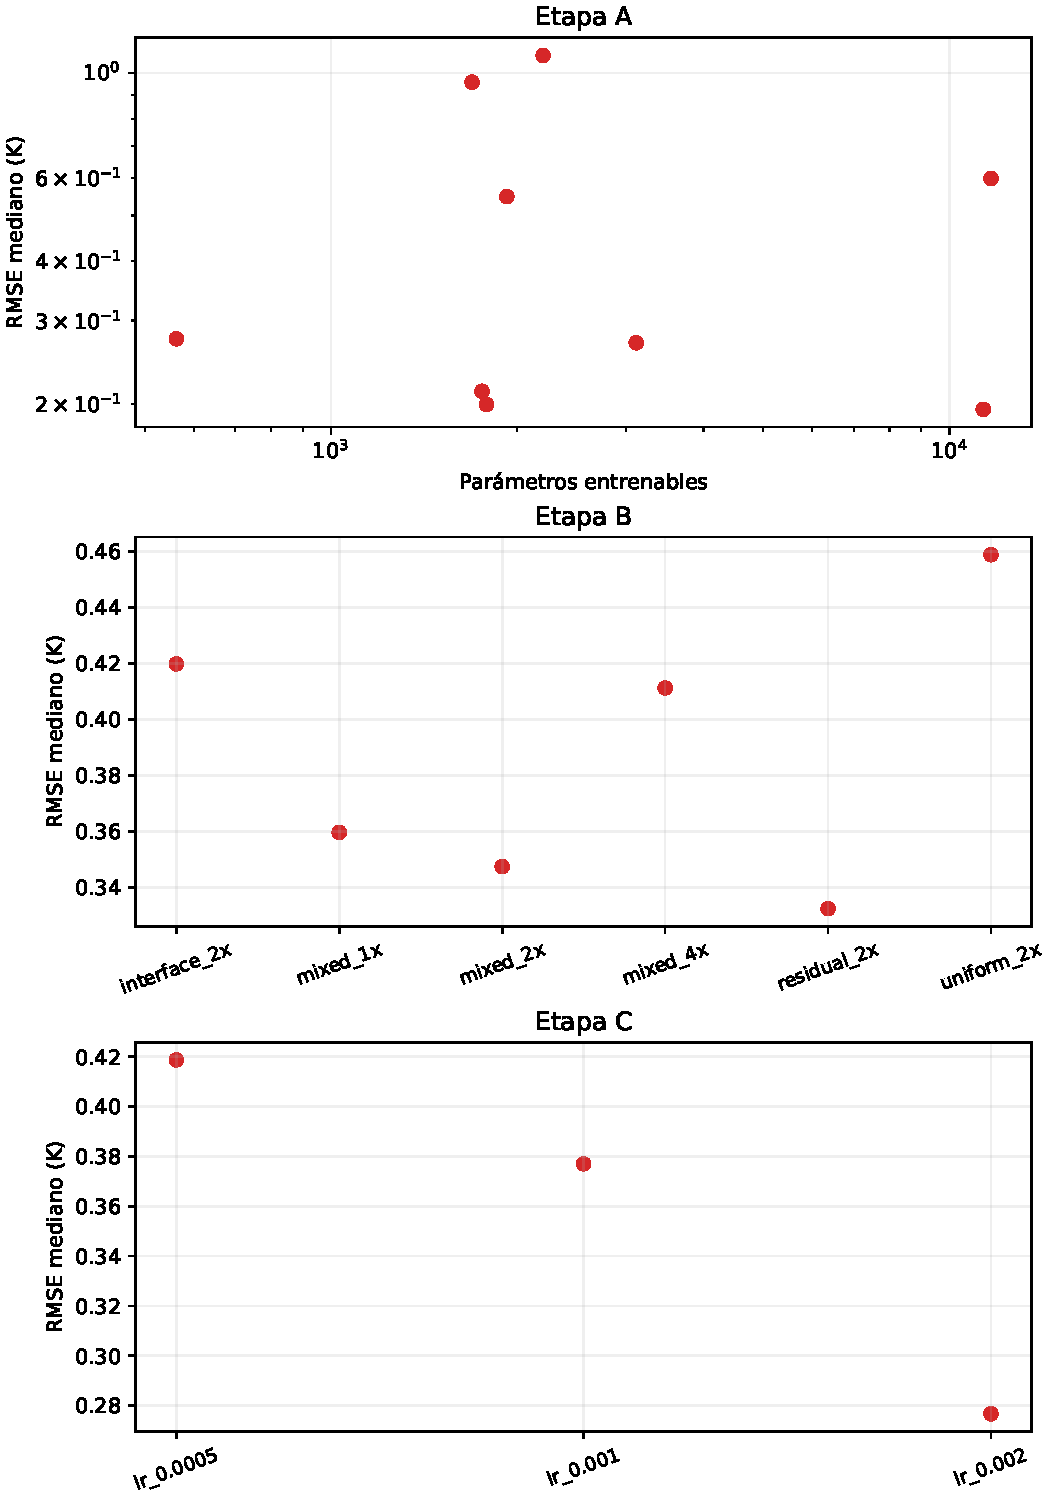
\includegraphics[width=.88\textwidth,height=.82\textheight,keepaspectratio]{explicit/selection.pdf}

\caption{Comparación de desarrollo. Verde: aceptación completa; rojo: al menos un rechazo. Los paneles corresponden a etapas distintas y no a un único factorial. Fuente: elaboración propia.}
\label{fig:explicit-selection}\end{figure}

\begin{figure}[htbp]\centering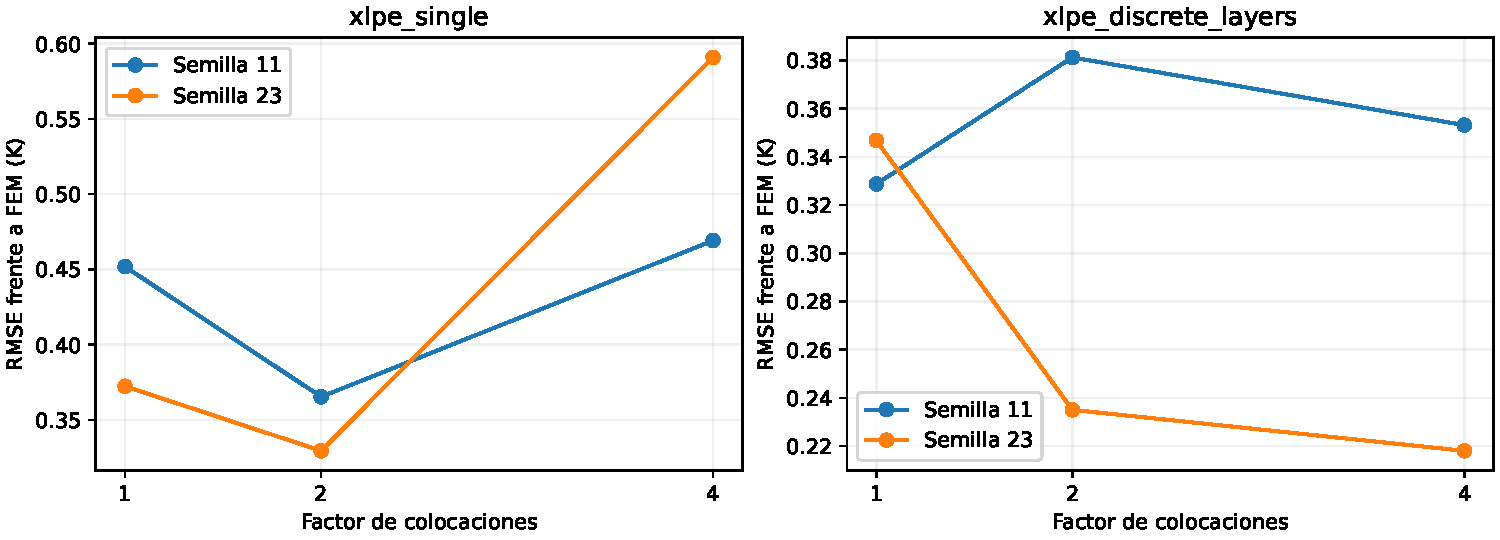
\includegraphics[width=\textwidth]{explicit/convergence.pdf}

\caption{Sensibilidad al número de colocaciones con la misma arquitectura y política geométrica. Fuente: elaboración propia.}
\label{fig:explicit-convergence}\end{figure}

\begin{figure}[p]\centering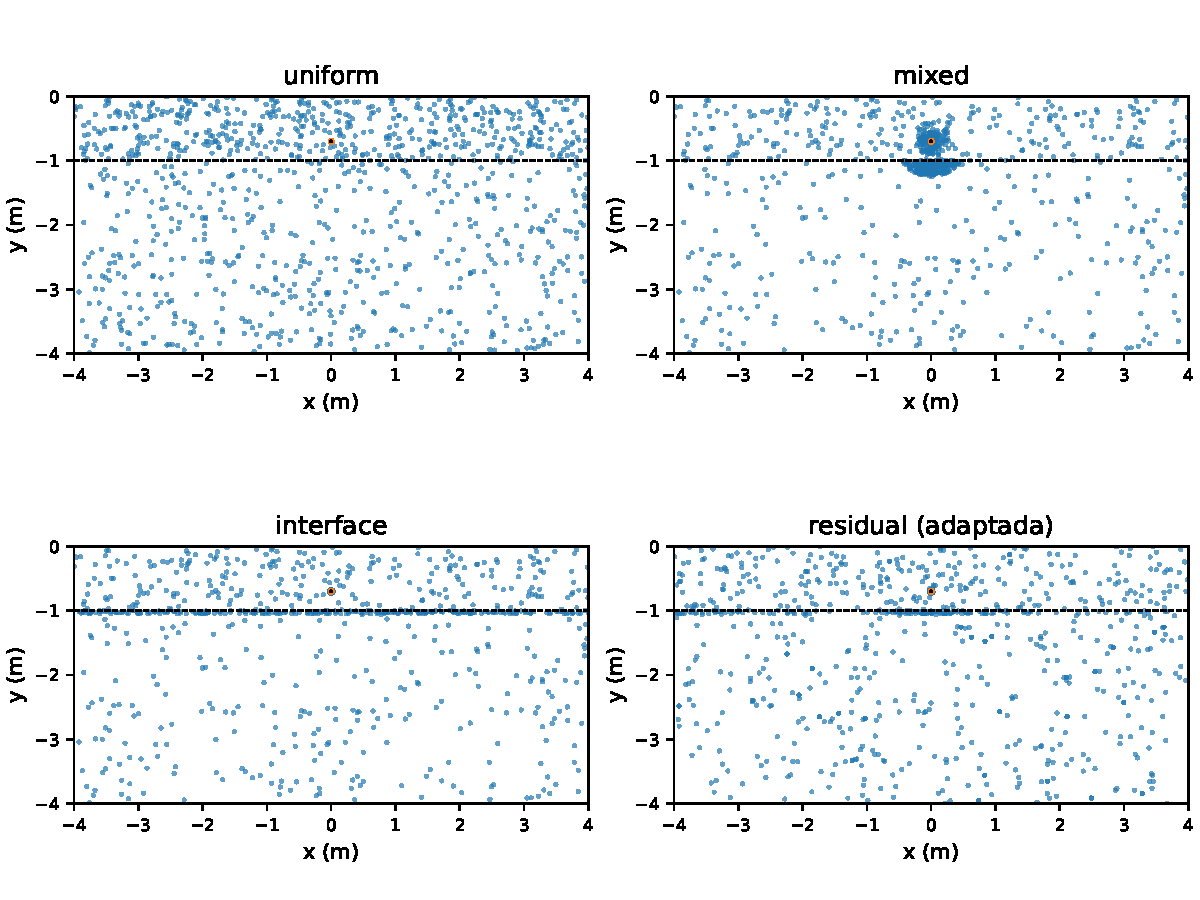
\includegraphics[width=\textwidth]{explicit/collocation_domain.pdf}

\caption{Cobertura del dominio para las cuatro políticas a igual presupuesto 2x, estratos y semilla 11. Azul: suelo; naranja: materiales del cable; líneas: interfaces geométricas. Se muestran colocaciones interiores, no las cuadraturas de trazas. Fuente: nubes archivadas; la política residual muestra la nube posterior a la adaptación.}
\label{fig:explicit-collocation-domain}\end{figure}

\begin{figure}[p]\centering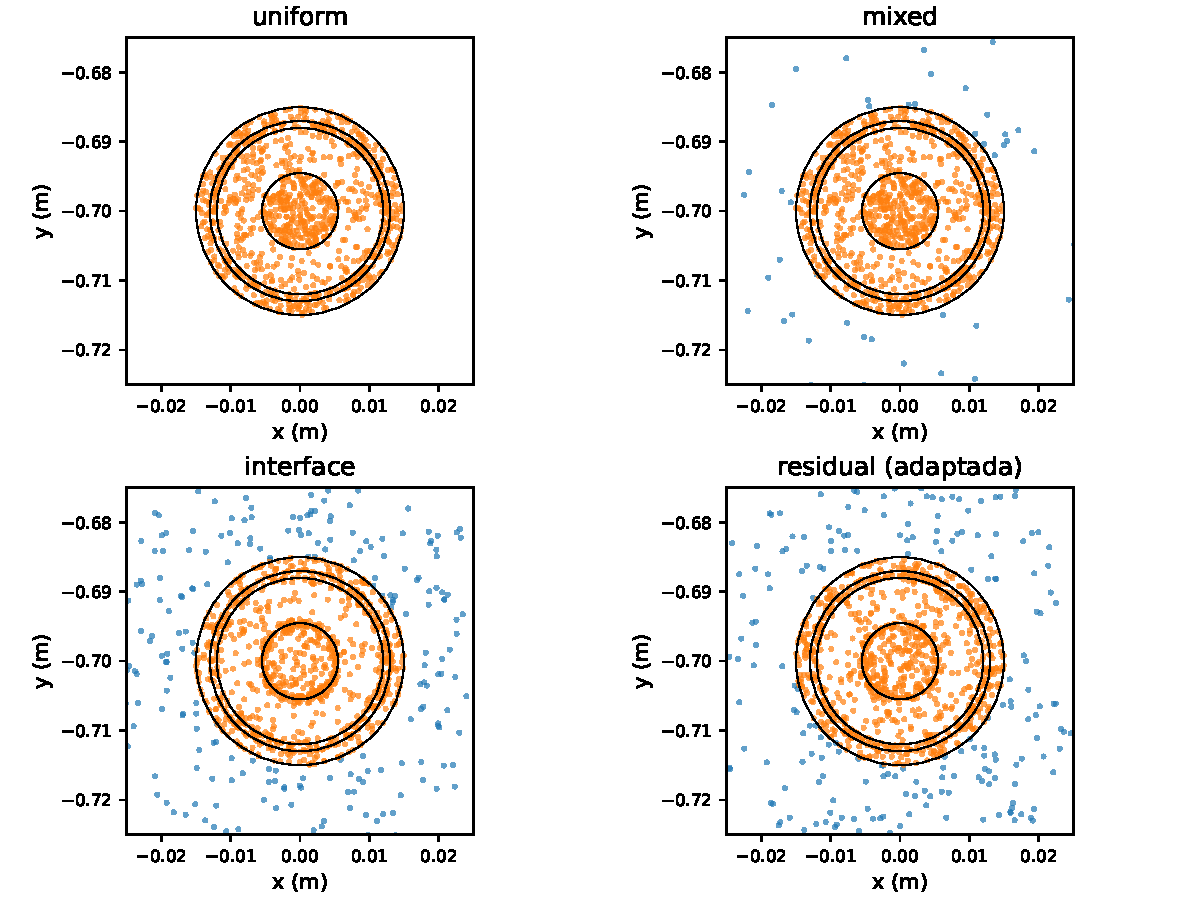
\includegraphics[width=\textwidth]{explicit/collocation_detail.pdf}

\caption{Detalle del cable para las cuatro políticas a igual presupuesto 2x, estratos y semilla 11. Azul: suelo; naranja: materiales del cable; líneas: interfaces geométricas. Se muestran colocaciones interiores, no las cuadraturas de trazas. Fuente: nubes archivadas; la política residual muestra la nube posterior a la adaptación.}
\label{fig:explicit-collocation-detail}\end{figure}

\begin{figure}[htbp]\centering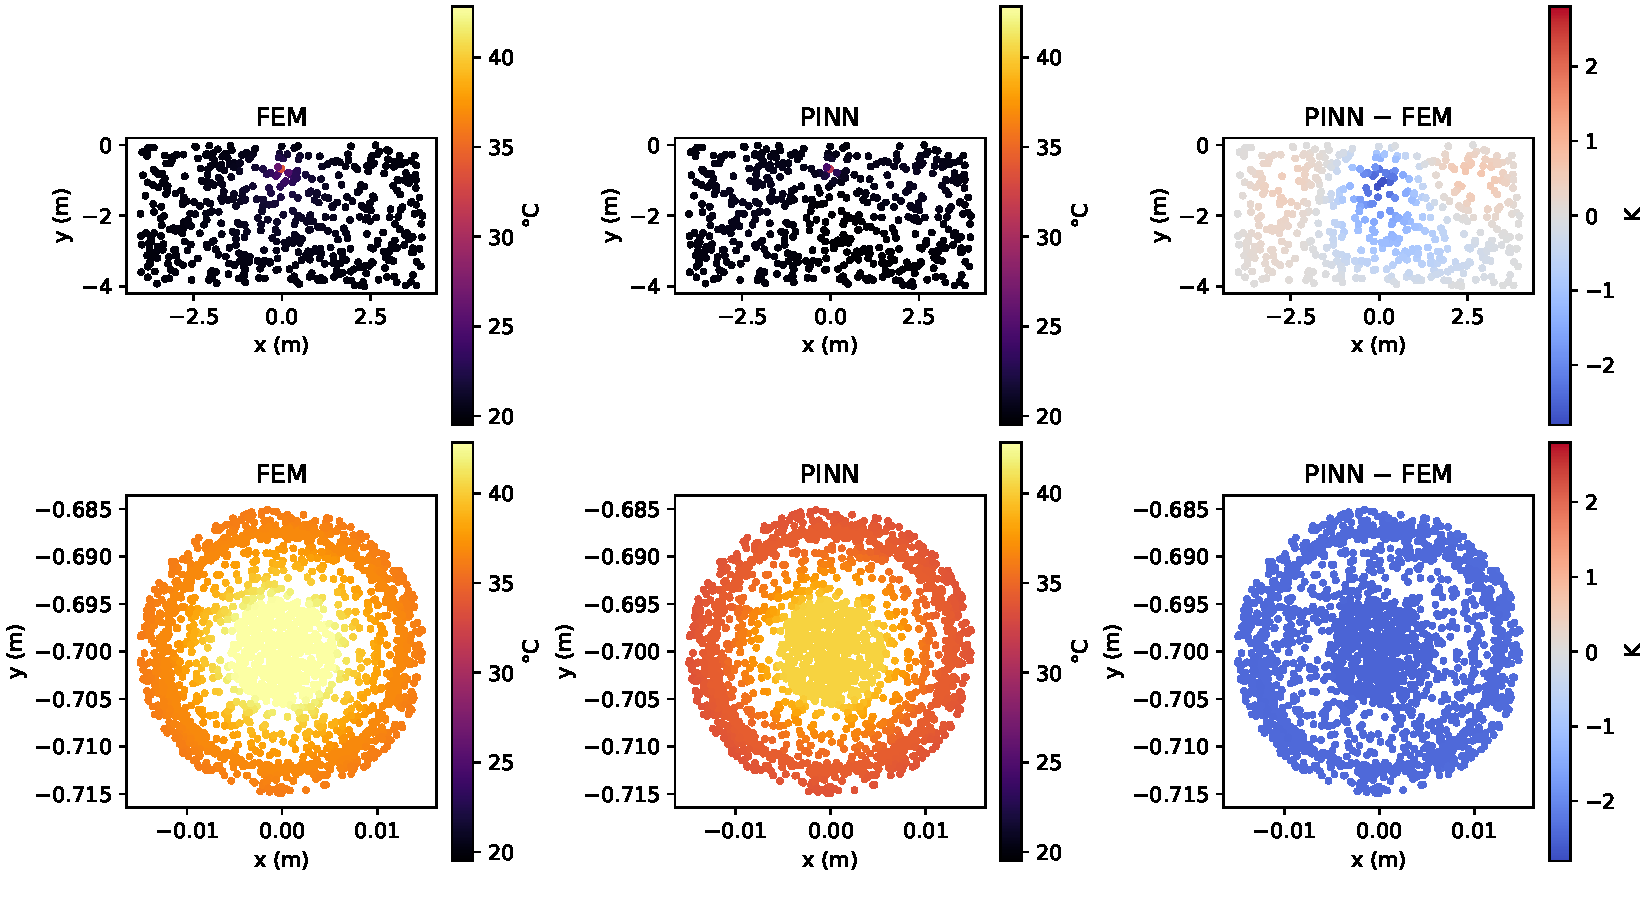
\includegraphics[width=\textwidth]{explicit/field.pdf}

\caption{Suelo y detalle interior del cable en XLPE con zona seca cercana, semilla 71 fijada previamente. Las temperaturas comparten escala y el error usa escala simétrica. Fuente: campos de confirmación.}
\label{fig:explicit-field}\end{figure}


\subsection{EFECTO PIEL Y DISTRIBUCIÓN INTERIOR DEL CALOR}

El cálculo cilíndrico condicional asume resistencia DC a \SI{20}{\celsius} y un conductor macizo homogéneo aislado. Entre \SI{20}{\celsius} y \SI{90}{\celsius}, el modelo estima incrementos de pérdidas por efecto piel de 0,195\,\pct{} a 0,317\,\pct{} en el cable XLPE pequeño, y de 25,578\,\pct{} a 37,136\,\pct{} en los conductores de mayor diámetro del catálogo. Estas cifras no certifican la resistencia AC efectiva de los cables comerciales referenciados, ya que dicha determinación exige conocer su construcción exacta, frecuencia y procedencia primaria.

En la verificación FEM 2D del caso Aras a potencia AC total equivalente se compararon cuatro niveles de malla para fuente uniforme y perfil radial por efecto piel. Al pasar de generación uniforme a perfil piel, la diferencia en $\Tmax$ resultó de $-0,004132$, $-0,004051$, $-0,004045$ y $-0,004045$ K conforme se refinaba la malla hasta alcanzar \num{380113} grados de libertad y un desequilibrio energético de 0,002402\,\pct{}. La convergencia entre los dos últimos refinamientos fue cercana a $4,1\times10^{-7}$ K, normalizando siempre la densidad de fuente interpolada por su integral numérica para aislar la redistribución espacial respecto de variaciones de potencia.

Esta comprobación indica que la redistribución radial interna del calor induce una variación térmica estacionaria inferior en más de un orden de magnitud al umbral de \SI{0,1}{\kelvin} empleado en la verificación. Sin embargo, el resultado no autoriza a omitir el factor de incremento de pérdidas totales entre DC y AC ni es extensible directamente a efectos de proximidad entre fases o transitorios rápidos. El módulo de fuente no uniforme permanece activo y la ecuación térmica se resuelve siempre en el interior metálico.

\subsection{ACOPLAMIENTO LOCAL Y ALCANCE DE LA AMPACIDAD}

El acoplamiento DC dependiente de temperatura descrito en la Sección~\ref{subsec:busqueda-ampacidad} se verificó en el control coaxial comparando la formulación explícita PINN frente a su referencia FEM fina. El modelo de elementos finitos alcanzó \SI{32,571582}{\celsius} y la PINN obtuvo \SI{32,575572}{\celsius}, lo que representa una discrepancia absoluta de \SI{0,003990}{\kelvin}. Este piloto confirma la correcta implementación matemática de la ley local de la Fórmula~\ref{for:fuente-dc-local}, pero no constituye una campaña completa de confirmación de ampacidad ni sustituye la búsqueda de corriente límite sobre escenarios heterogéneos. Asimismo, los operadores de almacenamiento temporal quedaron implementados sin haberse ejecutado simulaciones transitorias completas.

La búsqueda de corriente límite con la formulación explícita no se ha ejecutado y permanece pendiente. OE4 no se considera concluido con resultados de potencia fija ni con los de la formulación reducida anterior.


\subsection{DIAGNÓSTICO DE LOS RECHAZOS}
\label{sec:diagnostico-rechazos}

Un rechazo binario señala el incumplimiento de al menos una puerta numérica sin precisar el mecanismo limitante en cada caso. Para identificar el criterio restrictivo en la etapa D, se calcula la razón entre cada métrica observada y su tolerancia preinscrita en la Sección~\ref{sec:seleccion-pinn}. Los cocientes comparan el máximo entre NRMSE y RMSE por material frente al 5\,\pct{}, el error de $\Tmax$ frente al 5\,\pct{}, el desequilibrio energético frente al 2\,\pct{}, el salto térmico de interfaz frente a \SI{0,1}{\kelvin} y el salto RMS de flujo frente al 1\,\pct{}. Todo cociente superior a la unidad representa un incumplimiento, y la Tabla~\ref{tab:explicit-D-diagnosis} recoge el valor máximo obtenido entre las tres semillas de confirmación por problema.

\begin{table}[htbp]
\centering
\caption{Etapa D: razón máxima entre el valor observado y la tolerancia, por criterio y problema (máximo entre las tres semillas). Un valor mayor que 1 incumple el criterio. Fuente: elaboración propia a partir de los registros de confirmación.}
\label{tab:explicit-D-diagnosis}
\setlength{\tabcolsep}{3pt}
\begin{tabularx}{\textwidth}{L{3.2cm}C{1.1cm}C{1.3cm}C{1.1cm}C{1.5cm}C{1.3cm}C{1.4cm}Y}
\toprule
Problema & Acept. & Campo & $T_{\max}$ & Energía & Salto de $T$ & Salto de flujo & Criterio dominante \\
\midrule
xlpe\_single & 3/3 & 0,45 & 0,45 & 0,44 & 0,31 & 0,55 & Ninguno \\
xlpe\_dry\_far & 3/3 & 0,52 & 0,52 & 0,48 & 0,27 & 0,53 & Ninguno \\
xlpe\_dry\_near & 1/3 & 2,16 & 2,16 & 0,86 & 0,40 & 0,59 & $T_{\max}$ y campo \\
xlpe\_backfill & 0/3 & 1,99 & 1,99 & 1,46 & 0,28 & 0,95 & $T_{\max}$ y campo \\
xlpe\_discrete\_layers & 0/3 & 0,92 & 0,92 & 0,52 & 1,70 & 1,88 & Salto de flujo y de $T$ \\
aras\_flat & 0/3 & 16,21 & 5,54 & 0,12 & 1,18 & 0,59 & Campo \\
kim\_sand & 0/3 & 6,29 & 5,75 & 1,34 & 2,51 & 2,02 & Campo y $T_{\max}$ \\
\bottomrule
\end{tabularx}
\end{table}

Los mecanismos de fallo difieren según la complejidad física del caso. En el caso plano de Aras y en la configuración de Kim en arena, el error del campo térmico supera en 16,21 y 6,29 veces el umbral permitido respectivamente, evidenciando incapacidad de la receta congelada para representar geometrías multicable bajo ese presupuesto. En el relleno mejorado y en la zona seca cercana, la limitación principal radica en el error de $\Tmax$ y del campo con cocientes máximos de 1,99 y 2,16. Sin embargo, la semilla 83 de la zona seca cercana alcanzó un cociente de 0,76, mostrando sensibilidad a la inicialización aleatoria. Por el contrario, en los estratos discontinuos el campo y $\Tmax$ permanecen por debajo de la unidad (0,92), localizándose el rechazo exclusivamente en la transmisión de interfaz con saltos de flujo de 1,88 veces la tolerancia y de temperatura de 1,70 veces el umbral.

El diagnóstico de las etapas de calibración C y C2 presentado en la Tabla~\ref{tab:explicit-C-diagnosis} exhibe un compromiso equivalente entre restricciones. En la etapa C, la discontinuidad térmica en las interfaces dominó el rechazo en todas las tasas de aprendizaje evaluadas, alcanzando razones entre 4,42 y 5,13 frente al umbral de \SI{0,1}{\kelvin}. Al elevar la ponderación $w_T$ en la etapa C2 se redujo drásticamente el salto térmico hasta 0,23 veces la tolerancia para $w_T=10000$, pero la penalización desplazó el error hacia el salto de flujo normal (2,07 veces la cota). Ninguna combinación superó las cuatro corridas simultáneas de desarrollo, por lo que la receta seleccionada ($w_T=1000$, tasa $5\times10^{-4}$) constituye la mejor alternativa según la regla de preferencia y no un ajuste óptimo garantizado.

\begin{table}[htbp]
\centering
\caption{Etapas C y C2: razón máxima entre el valor observado y la tolerancia, por candidato (máximo entre las cuatro corridas de desarrollo). El candidato $w_T=100$ de C2 reutiliza las corridas de C con tasa $5\times10^{-4}$. Fuente: elaboración propia a partir de los registros de desarrollo.}
\label{tab:explicit-C-diagnosis}
\setlength{\tabcolsep}{3pt}
\begin{tabularx}{\textwidth}{L{3.2cm}C{1.1cm}C{1.3cm}C{1.1cm}C{1.5cm}C{1.3cm}C{1.4cm}Y}
\toprule
Etapa y candidato & Acept. & Campo & $T_{\max}$ & Energía & Salto de $T$ & Salto de flujo & Criterio dominante \\
\midrule
C, tasa $5\times10^{-4}$ ($w_T=100$) & 2/4 & 0,71 & 0,67 & 0,45 & 4,49 & 1,22 & Salto de $T$ \\
C, tasa $10^{-3}$ & 1/4 & 0,70 & 0,69 & 0,43 & 4,42 & 1,07 & Salto de $T$ \\
C, tasa $2\times10^{-3}$ & 1/4 & 0,52 & 0,22 & 0,30 & 5,13 & 1,15 & Salto de $T$ \\
C2, $w_T=1000$ & 2/4 & 0,80 & 0,80 & 0,43 & 1,60 & 1,56 & Salto de $T$ \\
C2, $w_T=10000$ & 2/4 & 0,57 & 0,57 & 0,35 & 0,23 & 2,07 & Salto de flujo \\
\bottomrule
\end{tabularx}
\end{table}

\subsection{DOMINIO DE ACEPTACIÓN}
\label{sec:dominio-validez}

El dominio de aceptación queda constituido exclusivamente por los problemas físicos en los cuales la receta congelada satisfizo la totalidad de los criterios numéricos y de conservación en las tres semillas nuevas de confirmación. La Tabla~\ref{tab:dominio-aceptacion} delimita este alcance para el dominio rectangular de $8\times4$ m con borde exterior a \SI{20}{\celsius}, entendiendo que cada configuración aceptada exige reentrenamiento específico y no transfiere pesos a otras geometrías ni conductividades.

También conviene contrastar estas cifras de confirmación frente a los umbrales de verificación fijados en la matriz del plan (Sección~\ref{subsec:proposiciones-diseno} y Tabla~\ref{tab:criterios-evaluacion}). En esa comparación, el cable XLPE homogéneo (error máximo de $\Tmax$ de \SI{0,378}{\kelvin} y $\mathrm{NRMSE}\leq 1,524\,\pct{}$) y la zona seca lejana (error máximo de \SI{0,441}{\kelvin} y $\mathrm{NRMSE}\leq 2,002\,\pct{}$) cumplen tanto la puerta del 5\,\pct{} como los requisitos de escenarios F3 del plan ($E_T<\SI{0,5}{\kelvin}$ y $\mathrm{NRMSE}<2,5\,\pct{}$). En cambio, ninguna corrida confirmada satisface la cota más estricta de referencia F2 ($E_T<\SI{0,1}{\kelvin}$ y $\mathrm{NRMSE}<1\,\pct{}$), lo cual refuerza el mantenimiento de las verificaciones FEM independientes como control obligatorio.

\begin{table}[htbp]
\centering
\caption{Dominio de aceptación de la receta congelada según la confirmación con semillas nuevas. Fuente: elaboración propia a partir de la Tabla~\ref{tab:explicit-production} y del diagnóstico de la Sección~\ref{sec:diagnostico-rechazos}.}
\label{tab:dominio-aceptacion}
\begin{tabularx}{\textwidth}{L{3.4cm}C{1.5cm}L{2.6cm}Y}
\toprule
Problema & Semillas aceptadas & Estado & Condición de uso \\
\midrule
xlpe\_single & 3/3 & Aceptado & Un cable XLPE en suelo homogéneo, con fuente prescrita. \\
xlpe\_dry\_far & 3/3 & Aceptado & Igual, con zona seca de $k=0,5$ W/(m K) a 1 m del eje. \\
xlpe\_dry\_near & 1/3 & Restringido & Resultado no reproducible entre semillas; requiere verificación con FEM antes de cualquier uso. \\
xlpe\_backfill & 0/3 & No aceptado & Candidato a la ronda E. \\
xlpe\_discrete\_layers & 0/3 & No aceptado & Candidato a la ronda E; el límite es la continuidad en la interfaz. \\
aras\_flat & 0/3 & No aceptado & No se reabre sin un cambio de arquitectura o de presupuesto que se justifique. \\
kim\_sand & 0/3 & No aceptado & Igual que el caso Aras plano. \\
\bottomrule
\end{tabularx}
\end{table}

La \emph{ronda E} constituye una fase formativa preinscrita y todavía no ejecutada para abordar los estratos discontinuos, el relleno mejorado y la zona seca cercana con semillas nuevas y los mismos criterios de aceptación. Su protocolo de intervención, incluyendo reglas de parada y registro íntegro de fallos, se encuentra documentado en \path{docs/PROTOCOLO_RONDA_E.md}, al igual que el protocolo preliminar de juicio de expertos descrito en el Anexo~\ref{anx:protocolo-expertos}. Hasta que ambas actividades sean ejecutadas, el dominio de validez permanece restringido a lo establecido en la Tabla~\ref{tab:dominio-aceptacion}.

\subsection{MATRIZ DE VALIDEZ}
\label{sec:matriz-validez}

La Tabla~\ref{tab:matriz-validez} delimita el alcance real de cada verificación efectuada, diferenciando explícitamente la verificación matemática de la validación física sobre instalaciones en servicio.

\begin{table}[htbp]
\centering
\caption{Matriz de validez de la evidencia. Fuente: elaboración propia a partir de las Tablas~\ref{tab:explicit-fem}, \ref{tab:explicit-production}, \ref{tab:explicit-effects} y~\ref{tab:explicit-effect-resolution}.}
\label{tab:matriz-validez}
\setlength{\tabcolsep}{3pt}
\begin{tabularx}{\textwidth}{L{2.7cm}Y Y Y}
\toprule
Qué se verifica & Contra qué referencia & Evidencia obtenida & Qué no establece \\
\midrule
Referencia FEM & Tres mallas por caso; cambio de $T_{\max}$ menor a 0,1 K y balance menor a 0,2\,\pct{} entre las dos últimas. & Mayor cambio de $T_{\max}$: 0,078 K; mayor balance: 0,027\,\pct{} (Tabla~\ref{tab:explicit-fem}). & Una cota del error exacto; propiedades reales, contornos o extensión del terreno. \\
Código FEM en simetría radial & Solución analítica coaxial. & Error de $T_{\max}$ de aproximadamente $3{,}68\times10^{-6}$ K. & Los casos angulares y heterogéneos. \\
Aceptación de la PINN & FEM de la misma formulación en puntos idénticos; seis criterios de la Sección~\ref{sec:seleccion-pinn}. & 7 de 21 ejecuciones aceptadas (Tabla~\ref{tab:explicit-production}). & Generalización a otros casos o a otras semillas; equivale a reentrenar por caso. \\
Efecto térmico de la heterogeneidad & Pares frente al XLPE homogéneo, a igual fuente prescrita. & Diferencias de $T_{\max}$ por caso (Tabla~\ref{tab:explicit-effects}). & Un efecto concluyente: ninguno satisfizo la regla de resolución preinscrita (Tabla~\ref{tab:explicit-effect-resolution}). \\
Contraste con valores publicados & Las geometrías de Aras (2005) y Kim (2025) se adoptan solo como configuración. & No se ha realizado con la formulación explícita. & Concordancia con las temperaturas publicadas: exige reproducir sus pérdidas, propiedades y contornos. \\
Ampacidad explícita & Búsqueda de corriente límite con la misma ley de pérdidas. & No ejecutada. & Cumplimiento de OE4 en la formulación explícita. \\
Validez de campo & Mediciones de instalaciones reales. & No realizadas. & Comportamiento de una instalación real. \\
\bottomrule
\end{tabularx}
\end{table}

El contraste directo con las temperaturas publicadas por \textcite{aras2005} y \textcite{kim2025} queda pendiente porque los casos incluidos en la Tabla~\ref{tab:explicit-fem} responden a fuentes prescritas, conductividades de suelo y contornos rectangulares definidos por el contrato de prueba, distintos de las instalaciones descritas en aquellas publicaciones.

\section{DISCUSIÓN E INTERPRETACIÓN DE LOS RESULTADOS}
\label{sec:discusion}

La cuestión central de la evaluación radica en establecer qué arquitectura y qué protocolo cumplen simultáneamente las ecuaciones diferenciales en cada subdominio, las leyes de continuidad en las interfaces y la concordancia frente a FEM dentro del dominio delimitado. La evidencia demuestra que un descenso en la pérdida global, un campo visualmente suave o una estimación cercana de $\Tmax$ resultan insuficientes si no se verifican el balance energético regional y el flujo derivado de la ley de Fourier. Al mismo tiempo, el rechazo de las redes de menor tamaño describe su limitación bajo el presupuesto fijo adoptado sin constituir una prueba de imposibilidad matemática.

El diseño secuencial por etapas redujo el costo computacional de la exploración, aunque impidió evaluar interacciones cruzadas entre la arquitectura de la etapa A, el muestreo de la etapa B y los pesos de la etapa C2. En consecuencia, los resultados deben interpretarse como una búsqueda controlada preliminar y no como una optimización global del espacio de hiperparámetros. De igual forma, las parejas de semillas permiten contrastes consistentes entre alternativas, pero dos o tres realizaciones no bastan para caracterizar colas estadísticas de fallo poco frecuentes. En cuanto a la referencia FEM, los estudios de malla acotan la incertidumbre numérica de discretización, sin incorporar la variabilidad intrínseca de conductividades reales, resistencias de contacto o migración de humedad.

Los resultados de la etapa D admiten tres conclusiones interpretativas principales. En primer término, la receta congelada alcanza reproducibilidad completa en los dos problemas de menor complejidad geométrica y heterogeneidad moderada o lejana (\texttt{xlpe\_single} y \texttt{xlpe\_dry\_far}). En segundo lugar, la tasa de aceptación se degrada cuando aparecen interfaces extensas de conductividad discontinua, inclusiones de alto contraste cercanas al conductor o arreglos multifase complejos, identificándose exactamente mediante la Sección~\ref{sec:diagnostico-rechazos} qué criterio físico limita cada configuración. En tercer término, las diferencias de temperatura inducidas por las heterogeneidades (Tabla~\ref{tab:explicit-effects}) no superan la regla de resolución preinscrita frente a la dispersión entre semillas y la incertidumbre de malla (Tabla~\ref{tab:explicit-effect-resolution}), impidiendo atribuir dichos efectos de forma concluyente al solucionador PINN.

Por tanto, el conteo agregado de 7 ejecuciones aceptadas sobre 21 en la etapa D no representa una probabilidad empírica sobre una población de circuitos reales, sino el mapa de desempeño reproducible sobre siete casos discretos. El aporte metodológico del paradigma DSR radica precisamente en haber explicitado una física común verificable, exigido la consistencia del flujo derivado $-k\nabla T$, separado estrictamente desarrollo de confirmación y preservado los casos rechazados como insumos diagnósticos para futuras iteraciones. Finalmente, tanto el cálculo transitorio mediante el término de almacenamiento $\rho c_p T_t$ como la estimación de ampacidad normativa AC requieren desarrollos adicionales verificados antes de extraer conclusiones operativas sobre OE4.

\section{ESTIMACIÓN DEL IMPACTO DE LA SOLUCIÓN}
\label{sec:impacto}

El impacto alcanzado es principalmente metodológico y computacional: provee un contrato físico auditable entre PINN y FEM, elimina comparaciones sesgadas heredadas de modelos reducidos, automatiza la trazabilidad entre código y resultados y delimita con rigor los casos aceptados y rechazados. En el plano profesional, el procedimiento ofrece un criterio preventivo para descartar estimaciones neuronales que violen balances energéticos o continuidad de flujo, sin atribuir ahorros económicos ni superioridad de velocidad frente a los métodos de elementos finitos sin registros aislados comparativos de tiempo.

\subsection{VIABILIDAD TÉCNICA Y COSTO COMPUTACIONAL}

La Tabla~\ref{tab:costo-computacional} desglosa el costo de entrenamiento de confirmación en la etapa D por caso y semilla. Una corrida en el cable XLPE monocapa requirió entre 8 y 11 minutos, mientras que el caso Aras plano demandó cerca de 21 minutos y el problema multicable de Kim alcanzó aproximadamente 92 minutos por semilla debido al incremento hasta \num{125038} parámetros entrenables. Las 101 ejecuciones acumuladas en las etapas A--D totalizaron 15,0 horas de cómputo acumulado en CPU, correspondiendo 8,0 horas a la etapa D bajo hasta tres procesos concurrentes en doble precisión. Dado que la concurrencia introduce competencia por recursos y que no se cronometraron corridas equivalentes aisladas de FEniCSx, estos registros describen el esfuerzo computacional invertido sin establecer ventaja temporal frente a FEM.

\begin{table}[htbp]
\centering
\caption{Costo computacional por corrida de confirmación (etapa D, tres semillas por problema). Fuente: elaboración propia a partir de los registros de confirmación.}
\label{tab:costo-computacional}
\begin{tabularx}{\textwidth}{L{3.6cm}C{2.2cm}C{1.7cm}C{1.7cm}C{1.7cm}Y}
\toprule
Problema & Parámetros entrenables & Mínimo, s & Mediana, s & Máximo, s & Aceptadas \\
\midrule
xlpe\_single & 11338 & 496 & 505 & 505 & 3/3 \\
xlpe\_dry\_far & 11338 & 528 & 532 & 537 & 3/3 \\
xlpe\_dry\_near & 11338 & 513 & 514 & 516 & 1/3 \\
xlpe\_backfill & 11338 & 510 & 511 & 523 & 0/3 \\
xlpe\_discrete\_layers & 13612 & 656 & 672 & 675 & 0/3 \\
aras\_flat & 29530 & 1277 & 1278 & 1303 & 0/3 \\
kim\_sand & 125038 & 5487 & 5546 & 5560 & 0/3 \\
\bottomrule
\end{tabularx}
\end{table}

El análisis por resultado válido revela que más de dos tercios del tiempo invertido en la etapa de confirmación se destinó a las configuraciones multicable de Aras y Kim, donde ninguna semilla satisfizo todos los criterios. Este contraste confirma que el incremento de parámetros y tiempo de entrenamiento no garantiza la aceptación cuando persisten errores de campo o de transmisión en interfaces complejas.

\subsection{RIESGOS Y BENEFICIO--COSTO}

La Tabla~\ref{tab:matriz-riesgos} sintetiza los principales riesgos técnicos y metodológicos identificados durante el desarrollo y la ejecución del artefacto, junto con su nivel cualitativo de probabilidad, impacto y medidas de mitigación adoptadas o pendientes.

\begin{table}[htbp]
\centering
\caption{Matriz cualitativa de riesgos del artefacto y de su uso. Fuente: elaboración propia a partir de los resultados de la campaña.}
\label{tab:matriz-riesgos}
\begin{tabularx}{\textwidth}{L{3.6cm}C{1.8cm}C{1.5cm}Y}
\toprule
Riesgo & Probabilidad & Impacto & Mitigación \\
\midrule
Rechazo del artefacto en configuraciones de interés (7 de 21 ejecuciones aceptadas). & Alta & Alto & Declarar el dominio de aceptación; ejecutar la ronda E; verificar con FEM antes de usar. \\
Uso fuera del dominio aceptado como si fuera una certificación. & Media & Alto & La etiqueta ``producción'' no certifica; la matriz de validez y la conservación de rechazos delimitan el uso. \\
Variabilidad entre semillas con solo dos o tres repeticiones. & Media & Medio & Informar mediana, rango y cantidad aceptada; confirmar con semillas nuevas. \\
Costo de los problemas grandes (Kim, 92 minutos por corrida). & Media & Medio & Presupuestos declarados; no ampliar sin una razón física o numérica. \\
Cambios de versión del software (FEniCSx, Gmsh, PyTorch). & Media & Medio & Versiones y huellas registradas en cada expediente; fijar rangos de dependencias queda pendiente. \\
Leer la ampacidad no ejecutada como resultado. & Media & Alto & OE4 se declara no alcanzado en la formulación explícita; no se afirma corriente admisible. \\
\bottomrule
\end{tabularx}
\end{table}

Desde la perspectiva beneficio--costo, la solución aporta un procedimiento reproducible, criterios de rechazo cuantitativos y trazabilidad completa entre modelos físicos y resultados numéricos. En contrapartida, sus costos comprenden las 15,0 horas de entrenamiento acumuladas en la campaña, el esfuerzo de preparar referencias FEM refinadas en tres mallas y la necesidad de reentrenar las subredes para cada caso nuevo. En consecuencia, el balance resulta cualitativamente favorable por rigor metodológico y control de calidad, sin sustentar ahorros económicos directos ni ventajas de tiempo de ejecución.

\subsection{SOSTENIBILIDAD}

La ejecución de la investigación es autofinanciada y se apoya íntegramente en herramientas científicas de código abierto (FEniCSx, Gmsh, PETSc y PyTorch), evitando dependencias de licencias comerciales propietarias. El consumo eléctrico del equipo durante los entrenamientos no se registró, por lo que no se formulan afirmaciones sobre su huella energética operativa. La sostenibilidad técnica del repositorio descansa en la preservación de configuraciones, semillas y huellas SHA-256; la licencia preliminar del repositorio (\texttt{LICENSE.md}) se encuentra definida para revisión institucional previa a la publicación, en tanto que el acotamiento estricto de los rangos de versión de las dependencias queda pendiente. A partir de esta delimitación técnica y de los resultados confirmados, el Capítulo~\ref{ch:conclusiones} consolida las conclusiones por objetivo específico y las recomendaciones correspondientes.
